\documentclass{beamer}

\usepackage{default}
\usepackage{amssymb}
\usepackage[utf8]{inputenc}

\DeclareGraphicsExtensions{{.pdf},{.png},{.jpg}}
\graphicspath{ {./img/} }

\hypersetup{colorlinks,urlcolor=blue}
\AtBeginSection[]
{
	\begin{frame}
		\begin{NoHyper}
		\tableofcontents[currentsection]
		\end{NoHyper}
	\end{frame}
}
\begin{document}
\addtobeamertemplate{footline}{\insertframenumber/\inserttotalframenumber}

	
\title{Introduction to MCMC}
\author{Alberto Lumbreras}
\date{February 4, 2016}
\maketitle

\begin{frame}\frametitle{Overview} 
\begin{NoHyper}
\tableofcontents
\end{NoHyper}
\end{frame}

\section{Introduction to Bayesian inference}
\begin{frame}{Intro to Bayesian Inference (``inverse probability")}{A controversial formula}

	\begin{quote}
	{\color{red}``The theory of inverse probability is founded upon an error, and must be wholly rejected!"}  \text{\normalfont Fisher, 1925}
	\end{quote} 
	\begin{quote}
	{\color{red}``Reduces all probability to a subjective judgement."} \text{\normalfont Fisher, 1956} 
\end{quote} 
	\begin{quote}
	{\color{red}``Fallacious rubbish!"} \text{\normalfont Fisher about Laplace, 1958}
	\end{quote}

	\begin{quote}
	``The more I consider it, the more clearly it would appear that I have been doing almost exactly what Bayes had done in the 18th century."
	\text{\normalfont Fisher, 1959}
	\end{quote} 
\end{frame}

\begin{frame}{Intro to Bayesian Inference (``inverse probability" )}{Thomas Bayes' formula (one more time)}
	
	\begin{equation}
	\underbrace{p(\theta | y)}_{posterior} 
	= 
	\frac{\overbrace{p(y, \theta)}^{\text{joint probability}}}{\int_\theta p(y, \theta)}
	=
	\frac{\overbrace{p(y | \theta)}^{likelihood} \overbrace{p(\theta)}^{prior}}{\int_\theta p(y | \theta) p(\theta)}
	\propto 
	\overbrace{p(y | \theta)}^{likelihood} \overbrace{p(\theta)}^{prior}
	\end{equation}
	\begin{itemize}
		\item Imagine we want to use Bayes in a non-trivial problem...
		\item ...where the denominator is not tractable (\textbf{usually})
		\item ...but we can \textbf{always} evaluate the likelihood and the prior.
		\item How can I get access to the posterior? 
	\end{itemize}
\end{frame}


\begin{frame}{Intro to Bayesian Inference }{Computers to the rescue}
		\begin{equation}
		\underbrace{p(\theta | y)}_{posterior} 
		\propto 
		\overbrace{p(y | \theta)}^{likelihood} \overbrace{p(\theta)}^{prior}
		\end{equation}
		\begin{itemize}
			\item The denominator was just a normalizing factor.
			\item Therefore drawing samples from $\overbrace{p(y | \theta)}^{likelihood} \overbrace{p(\theta)}^{prior}$ is like drawing samples directly from the posterior.
			\item ``\textit{I wish I had an Intel Core i7} :\_(" \\Thomas Bayes, circa 1750.
		\end{itemize}
\end{frame}

\section{Basic Monte Carlo methods}
\begin{frame}{Inverse method}{Exploiting the Cumulative Distribution Function}

	\begin{enumerate}
		\item Get the CDF: $\mathbb{R} \rightarrow [0,1]$ 
		\item Draw samples from uniform distribution.
		\item Map uniform samples to final samples through $CDF^{-1}: [0,1] \rightarrow \mathbb{R}$ 
	\end{enumerate}
	\begin{figure}
		\centering
		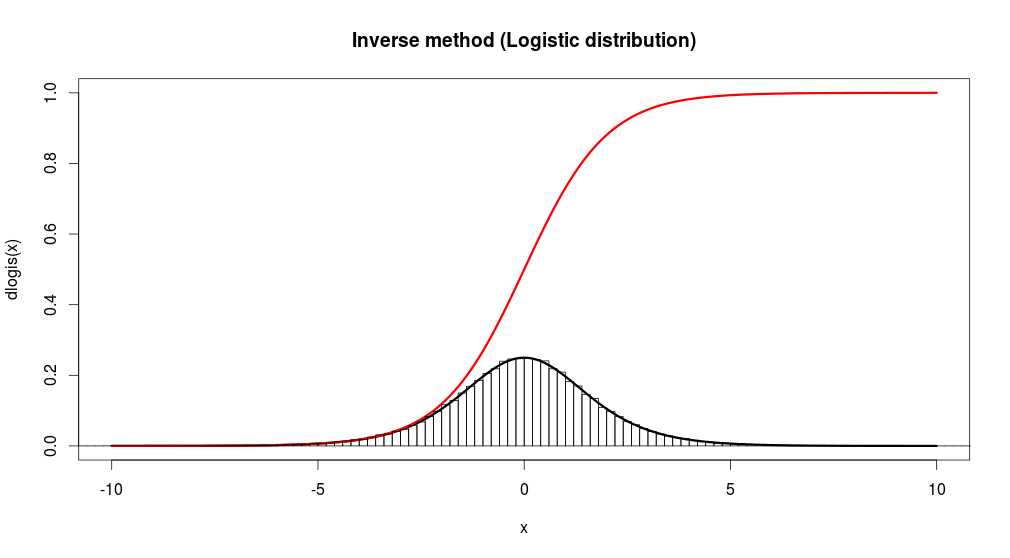
\includegraphics[width=\textwidth]{inverse.png}
	\end{figure}
\end{frame}

\begin{frame}{Inverse method}{Pros and cons}
	Pros:
		\begin{itemize}
			\item Faster possible method.
		\end{itemize}
	Cons:
	\begin{itemize}
		\item We don' have the CDF of most distributions.
		\item Only for unidimensional distributions.
	\end{itemize}

\end{frame}

\begin{frame}{Accept-Reject sampling}{Sample from a comfort zone}
	\begin{enumerate}
		\item Look for some pretty density $q$ that you know how to can sample from.
		\item Make it bigger than your ugly density $p$. ($Kq$)
		\item Draw sample $x_i$ from the pretty one.
		\item Accept samples with probability $p(x_i)/(Kq(x_i))$
	\end{enumerate}
		\begin{figure}
			\centering
			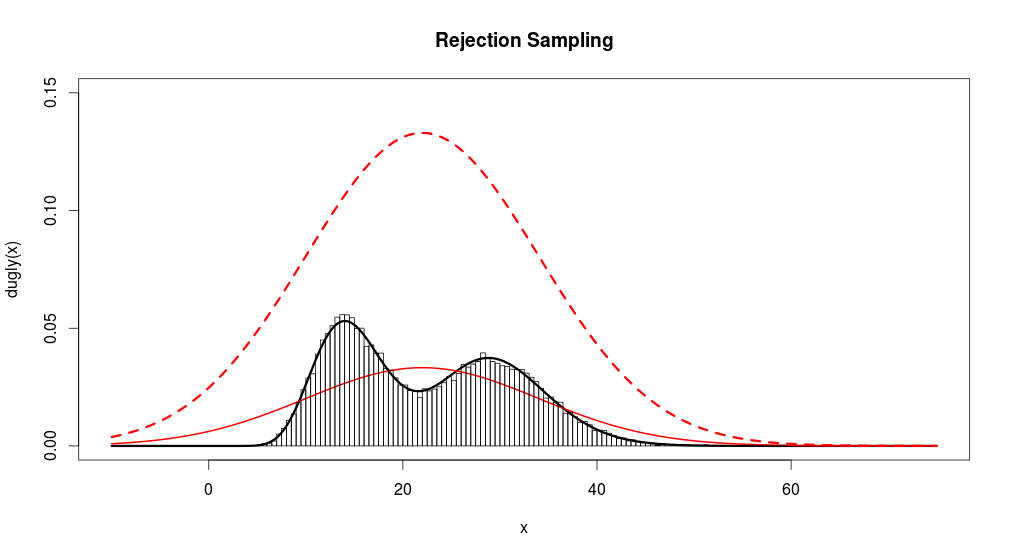
\includegraphics[width=\textwidth]{rejection.png}
		\end{figure}
\end{frame}

\begin{frame}{Accept-Reject sampling}{Pros and cons}
	Pros:
	\begin{itemize}
		\item We can usually find a pretty envelope $Kq$.
	\end{itemize}
	Cons:
	\begin{itemize}
		\item If $Kq$ is too wide or too big, lots of wasted (rejected) samples.
		\item Not always easy to find a good $Kq$.	\end{itemize}
\end{frame}

\section{Markov Chain Monte Carlo methods}
\begin{frame}{Metropolis-Hastings}{Jumping from last sample}
	\begin{enumerate}
		\item Start at some initial sample $x_0$
		\item Random jump $x_{i+1} \sim x_i + \mathcal{N}(0,step)$
		\item Accept with probability $p(x_{i+1})/p(x_i)$. If rejected, $x_{i+1} = x_i$
		\item Repeat 2 and 3 $N$ times ($N$ is the length of your Markov Chain)
	\end{enumerate}

	\begin{figure}
		\centering
		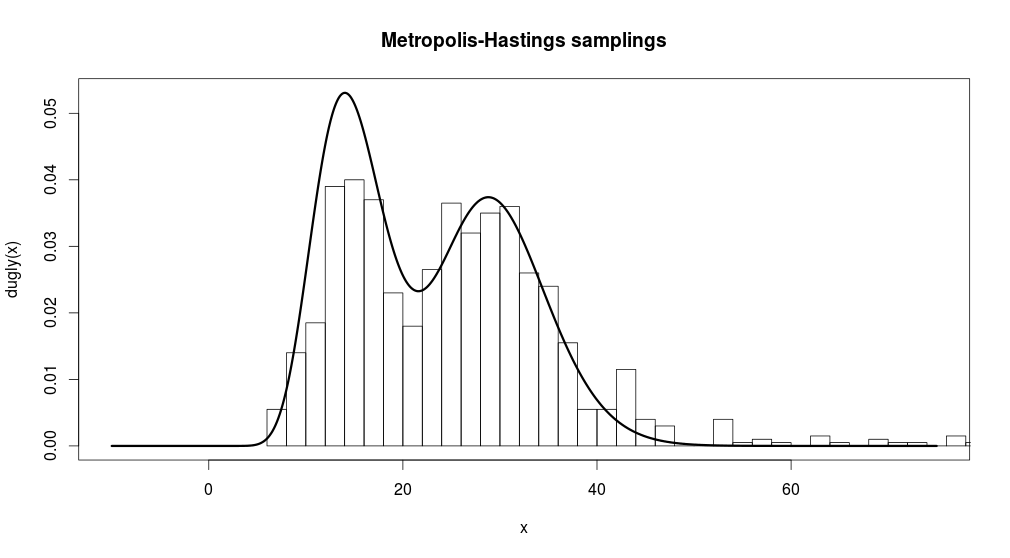
\includegraphics[width=\textwidth]{metropolis_unidimensional.png}
	\end{figure}
\end{frame}

\begin{frame}{Metropolis-Hastings}{About the Markov Chain}
	\begin{itemize}
		\item First samples depend on $x_0$. We drop them (burn-in).
		\item After burn-in, we are sampling from the true distribution.
		\item Statistical convergence checks (see \texttt{coda} package in R).
	\end{itemize}
	\begin{figure}
		\centering
		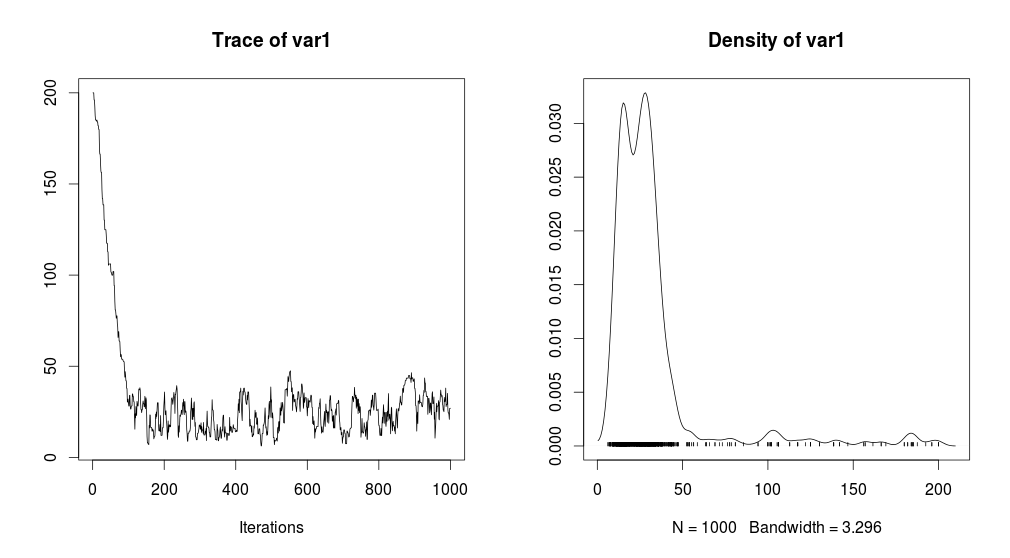
\includegraphics[width=\textwidth]{metropolis_traces.png}
	\end{figure}
\end{frame}

\begin{frame}{Metropolis-Hastings}{Pros and cons}
	Pros:
	\begin{itemize}
		\item Always works! (see ugly density below)
		\item Step size needs to be carefully tuned (for efficiency).
	\end{itemize}
	Cons:
	\begin{itemize}
		\item Rejects $\sim 70-80$\% of samples (recommended).
	\end{itemize}
	\begin{figure}
		\centering
		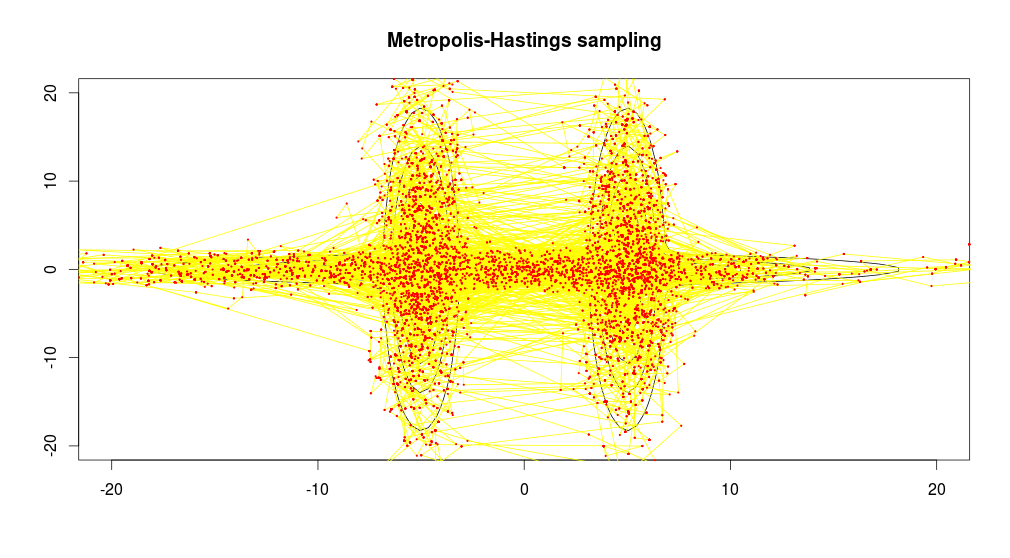
\includegraphics[width=\textwidth]{metropolis_bidimensional.png}
	\end{figure}
\end{frame}

\begin{frame}{Gibbs sampling}{Sample from pretty individual conditional probabilities.}
	Ugly $p(x1, x2, x3)$
	\begin{enumerate}
		\item Choose a initial $x_1, x_2, x_3$
		\item Draw $x_1 \sim p(x_1 | x_2, x_3)$ (easy!)
		\item Draw $x_2 \sim p(x_2 | x_1, x_3)$ (easy!)
		\item Draw $x_3 \sim p(x_2 | x_2, x_1)$ (easy!)
		\item Repeat 1,2 and 3 $N$ times.
	\end{enumerate}
		\begin{figure}
			\centering
			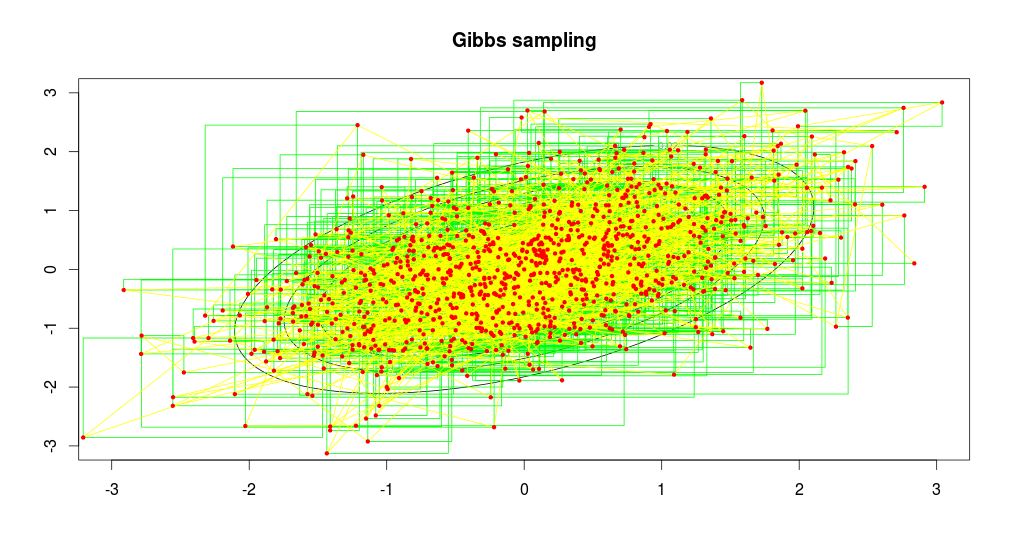
\includegraphics[width=\textwidth]{gibbs.png}
		\end{figure}
\end{frame}

\begin{frame}{Gibbs sampling}{Prons and cons}
	Pros:
	\begin{itemize}
		\item Just a smart Metropolis-Hastings where all samples are accepted.
	\end{itemize}
	Cons:
	\begin{itemize}
		\item Only possible if conditional probabilities are pretty.
		\item (... and for that we need to use \textit{conjugate priors})
	\end{itemize}
\end{frame}


\begin{frame}{Wrap-up}
	\begin{itemize}
	\item We sample because we can't do the maths analytically.
	\item Gibbs and Metropolis are a must in a Bayesian toolbox.
	\end{itemize}
	Caveat:
	\begin{itemize}
		\item burn-in can take toooo much.
	\end{itemize}
	Alternatives:
	\begin{itemize}
		\item Laplace approximations.
		\item\textbf{ Variational Inference (approximation)} (very popular, very scalable)
		\item Expectation Propagation (approximation).
		\item ...	
	\end{itemize}
\end{frame}
\begin{frame}{Readings}
	Historical debate:
	\begin{itemize}
			\item \href{http://projecteuclid.org/download/pdf_1/euclid.ba/1340370565}{Aldrich, \textit{R. A. Fisher on Bayes and Bayes' theorem }}
			\item  \href{http://www.phil.vt.edu/dmayo/PhilStatistics/b\%20Fisher\%20design\%20of\%20experiments.pdf}{Fisher. \textit{The Design of Experiments} (page 6) }
	\end{itemize}
	MC Books and tutorials
	\begin{itemize}
		\item \href{http://www.indiana.edu/~kruschke/DoingBayesianDataAnalysis/}{Kruschke. \textit{Doing Bayesian Data Analysis.}}
		\item Bishop. \textit{Pattern Recognition and Machine Learning} (ch.11)
		\item Robert et Casella. \textit{Méthodes de Monte Carlo avec R}. 
		\item \href{http://www.stat.columbia.edu/~gelman/book/}{Gellman. \textit{Bayesian Data Analysis}.}
		\item \href{http://camdavidsonpilon.github.io/Probabilistic-Programming-and-Bayesian-Methods-for-Hackers/}{Cam Davidson-Pilon. \textit{Bayesian Methods for Hackers}.}
	\end{itemize}
	Divulgation:
	\begin{itemize}
		\item \href{https://en.wikipedia.org/wiki/The_Lady_Tasting_Tea}{Salsburg, D.\textit{The lady tasting tea.}}
		\item \href{https://en.wikipedia.org/wiki/The_Signal_and_the_Noise}{Silver, N. \textit{The Signal and the Noise: Why So Many Predictions Fail --but Some Don't.}}
	\end{itemize}
\end{frame}
\end{document}